\chapter{Implementation}
	
	\label{sec:implementation}
	
	This chapter describes the implementation of the system in detail. First the
	electronics produced are described and followed by an explanation of the
	firmware which drives them. Finally, safety considerations and a brief
	discussion of the development methodology used is presented.
	
	\section{Electronics}
		
		Two circuits were produced, one which hosts the Mbed and the electronics
		needed to drive the heaters, motors and temperature sensors and another
		which provides an interface between the end-stops and stepper controller
		boards.
		
		The main board will host the Mbed, electronics for controlling heaters and
		motors, reading from temperature sensors and connections for the stepper
		controller boards (figure \ref{fig:electronicsDiagram}). A second board is
		used for the end-stop electronics as these parts may be replaced separately
		from the main electronics and connect via the existing stepper controller
		interface. The completed system, as installed in the printer, is shown in
		figure \ref{fig:electronicsPhoto} with the major components labelled.
		
		To keep the system easy to build requiring readily available tools, 0.1"
		spaced electronics were used throughout. These are easy to work with using
		only a standard soldering iron and basic tools. Components of this size can
		also be used for prototyping with a solderless breadboard.
		
		\begin{figure}
			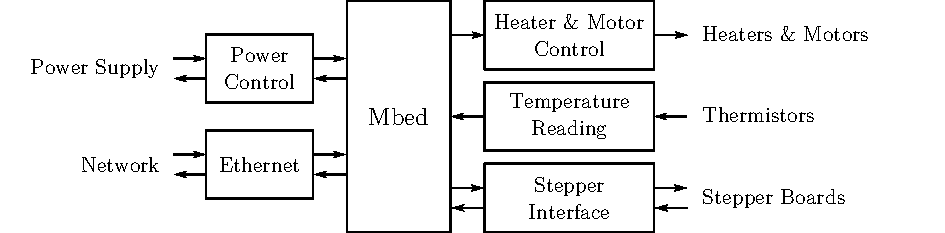
\includegraphics[width=1\textwidth]{diagrams/electronicsDiagram.pdf}
			\caption{Components of the main board}
			\label{fig:electronicsDiagram}
		\end{figure}
		
		\begin{figure}
			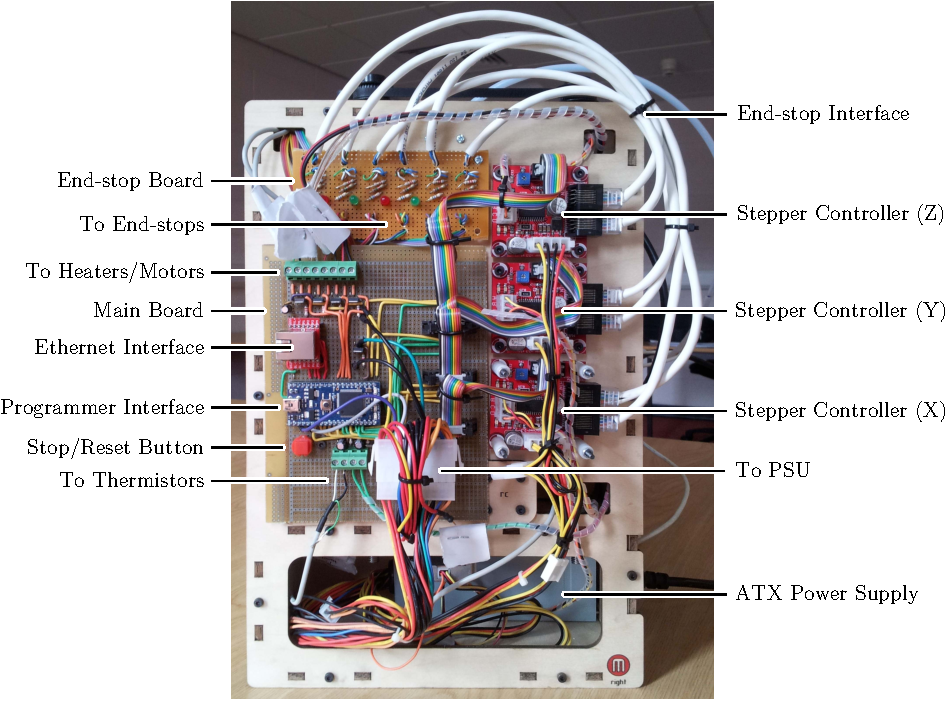
\includegraphics[width=1\textwidth]{diagrams/electronicsPhoto.pdf}
			\caption{Electronics installed with key components labelled}
			\label{fig:electronicsPhoto}
		\end{figure}
		
		\subsection{Layout \& Board}
			
			A prototyping board designed for working with DIP (Dual In-line Package)
			components such as the Mbed was selected (Figure \ref{fig:dipBoard}(B)).
			Conventional strip board (\ref{fig:dipBoard}(A)) is not ideal for these
			components as it would require many connections to be cut between the
			columns of pins. 
			
			\begin{figure}
				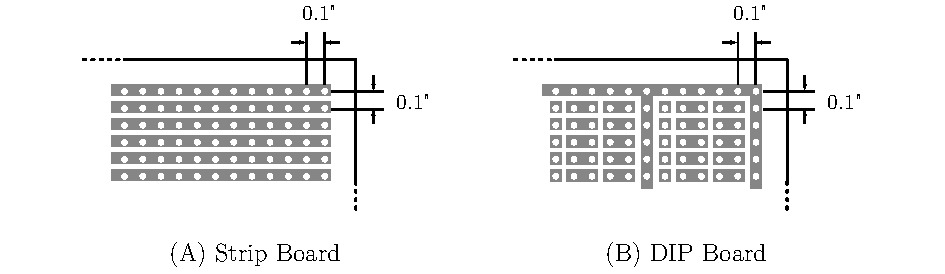
\includegraphics[width=1\textwidth]{diagrams/dipBoard.pdf}
				\caption{Types of prototyping board}
				\label{fig:dipBoard}
			\end{figure}
			
			\begin{figure}
				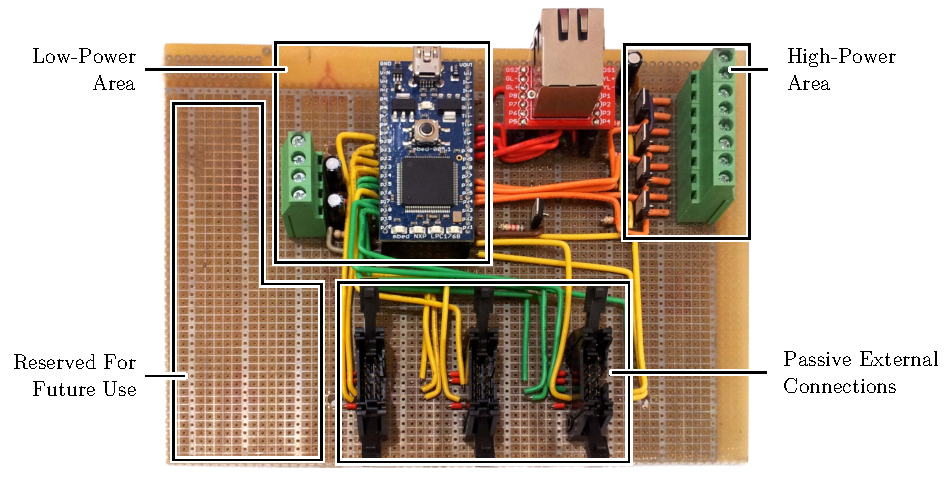
\includegraphics[width=1\textwidth]{diagrams/mainBoard.pdf}
				\caption{Top-level layout of main board (reset button and power
				         connections not shown)}
				\label{fig:mainBoard}
			\end{figure}
			
			The main board contains electronics for both low-power systems such as the
			Mbed and high-power systems such as the heater and motors and electrical
			interference between these parts must be minimised. The high and lower
			power parts have been kept physically separate on the board (figure
			\ref{fig:mainBoard}), each with their own power supply connections. The
			board also has a continuous track covering the whole board which can be
			connected to ground (known as a ground plane), helping reduce
			noise \cite{pcb_design_notes}.
			
			A full circuit schematic and pin-out for the board is given in Appendix
			\ref{sec:mainboardDiagrams}.
		
		\subsection{Heaters \& DC Motors}
			
			\label{sec:heatersAndMotors}
			
			The heaters and DC motors in the extruder and platform operate at a higher
			voltage and are considerably higher-current than the microcontroller can
			provide on its output pins. To control these a transistor can be used.
			Transistors act like a switch which allows high-power components to be
			switched on and off using only a small current from the Mbed. An
			IRLU8729PbF MOSFET (Metal Oxide Field Effect Transistor) was selected as
			it can switch large loads up to 58A with very little on-resistance
			(reducing energy wastage through heat) \cite{MOSFET}.
			
			\begin{figure}
				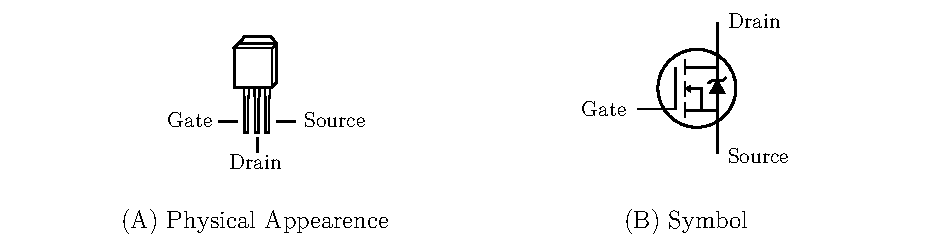
\includegraphics[width=1\textwidth]{diagrams/mosfetDiagram.pdf}
				\caption{Metal Oxide Semiconductor Field Effect Transistor (MOSFET)}
				\label{fig:mosfetDiagram}
			\end{figure}
			
			A MOSFET has three connections called the gate, drain and source
			(Figure \ref{fig:mosfetDiagram}). When the voltage between the gate and
			source is 0V, no current flows from the drain to the source. As the
			voltage between the gate and drain are increased, the current allowed to
			flow increases rapidly when it passes a certain threshold (Figure
			\ref{fig:mosfetPerformance}). By connecting the gate to a pin on the
			Mbed and the source to ground, a large current from a device such as a
			heater or motor attached to the drain can be switched.
			
			\begin{figure}
				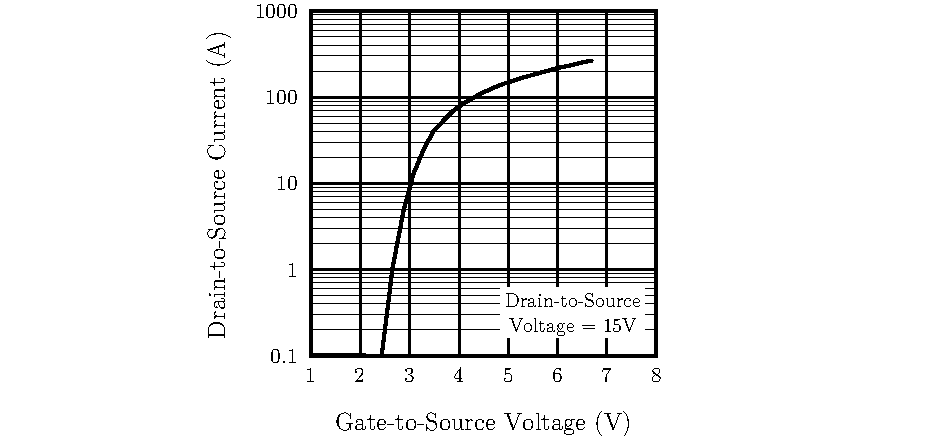
\includegraphics[width=1\textwidth]{diagrams/mosfetPerformance.pdf}
				\caption{IRLU8729PbF Typical Transfer Characteristics (reproduced from
				`Fig 3', \cite{MOSFET})}
				\label{fig:mosfetPerformance}
			\end{figure}
			
			The behaviour of a MOSFET when the gate is left floating (disconnected) is
			generally undefined and can damage the component. When the Mbed powers on
			its output pins default to a floating state which could cause a MOSFET to
			unexpectedly switch on or become damaged. To prevent this happening the
			gate is connected to ground via a resistor. When the output pin is
			floating the gate is pulled to 0V by the resistor. When the output of the
			pin is not floating, the gate is pulled to that voltage overriding the
			pull-down resistor. A high resistance value is used so that the Mbed can
			easily override the pull-down resistor. Figure \ref{fig:mosfetUsage} shows
			the circuit used to control the two heaters and two motors using a MOSFET
			and pull-down resistor.
			
			\begin{figure}
				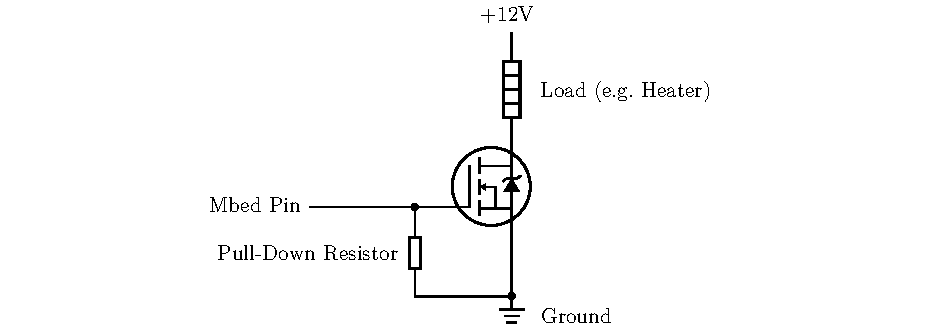
\includegraphics[width=1\textwidth]{diagrams/mosfetUsage.pdf}
				\caption{Example MOSFET circuit with pull-down resistor}
				\label{fig:mosfetUsage}
			\end{figure}
			
			When driving motors, a `flyback diode' is usually used to prevent a
			voltage spike occurring when the power is removed from the motor. This
			voltage spike is caused by the magnetic field in the motor's coils
			collapsing. This is not included in the circuit as the MOSFETs used
			already contain an appropriate diode.
			
			It should be noted that this circuit does not allow the motors to be
			driven in both directions as this is not needed by the printer. If this
			was required, a more complex circuit (such as an H bridge) would be
			needed.
		
		\subsection{Thermistors}
			
			\label{sec:thermistor}
			
			To measure the temperature of the heaters, thermistors are used. The
			resistance of a thermistor changes non-linearly with temperature and can
			be modelled using an equation derived from the Steinhart-Hart
			Equation \cite{Steinhart1968497}:
			\begin{equation}
				\frac{1}{T} = \frac{1}{T_0} + \frac{1}{\beta} \ln \left( \frac{R}{R_0} \right)
				\label{equ:steinhart}
			\end{equation}
			Where $T$ and $R$ are the current temperature and resistance of the
			thermistor, $T_0$ and $R_0$ are the temperature and resistance at a
			reference temperature and $\beta$ is a characteristic constant for the
			device available in the data-sheet.
			
			Using the Analog-to-Digital converter in the Mbed, voltages, but not
			resistances, can be read directly. As a result, a potential divider
			(figure \ref{fig:potentialDiv}) is used to produce a measurable voltage
			which is proportional to the resistance to measure it indirectly.
			\begin{figure}
				
\includegraphics[width=1\textwidth]{diagrams/potentialDiv.pdf}
				\caption{Potential divider}
				\label{fig:potentialDiv}
			\end{figure}
			A reference voltage $V_\textrm{ref}$ is placed across two resistors,
			$R_1$ and $R_2$, and the voltage between them at $V$ is measured. The
			relationship between these variables is
			\begin{equation}
				V = V_\textrm{ref} \frac{R_2}{R_1 + R_2}
			\end{equation}
			Thus, if the thermistor is placed as $R_2$, the resistance can be
			calculated using
			\begin{equation}
				R_2 = V_\textrm{ref} \frac{R_1}{V - V_\textrm{ref}}
				\label{equ:potdiv}
			\end{equation}
			
			The value of $R_1$ was chosen to evenly spread the voltages from the
			expected range of thermistor resistances over the full range of 0 to
			$V_\textrm{ref}$ volts. This maximises the utilisation of the analog to
			digital converter available over the temperature ranges used.
			
			Using (\ref{equ:steinhart}) and (\ref{equ:potdiv}) with a potential
			divider circuit will allow the temperature of the thermistor to be
			measured.
			
		
		\subsection{Stepper Motors}
			
			The stepper controllers chosen accept TTL signals and connect via a
			ten-pin insulation displacement connector (IDC). An IDC socket was
			placed on the board and the pins connected directly to the Mbed and
			ground plane as required.
		
		\subsection{End-stops}
			
			Optical end-stops consist of a photo-interrupter containing an infra-red
			LED and a photo-transistor arranged across a gap (Figure
			\ref{fig:endstop}). Photons from the LED activate the photo-transistor
			allowing current to flow but, when the gap is blocked, the transistor is
			switched off and no current flows.
			
			\begin{figure}
				
\includegraphics[width=1\textwidth]{diagrams/endstop.pdf}
				\caption{Photo-interrupter with a photo-transistor in a Darlington pair}
				\label{fig:endstop}
			\end{figure}
			
			Due to problems sourcing the interface boards for the end-stops, a circuit
			was built which is compatible with the stepper-controller interface. $+5V$
			and ground are provided and a TTL logic signal is expected by the
			interface. To ease debugging, an indicator LED was also added which is lit
			when the end-stop is unobstructed.
			
			The LED in the photo-interrupter is driven via a current-limiting
			resistor and the signal output and indicator LED are connected through
			the photo-transistor. A pull-down resistor is used to pull the signal
			to ground when the photo-transistor is powered off.
			
			The circuitry is placed on a board with cables running to each end-stop
			(shown mounted in figure \ref{fig:endstopInstalled}) and to each of the
			CAT-5 sockets on the stepper controller boards. Strain-relief is included
			so that the connections are not damaged if the cables are caught in the
			machine. A circuit diagram is provided in appendix
			\ref{sec:endstopDiagram}.
			
			\begin{figure}
				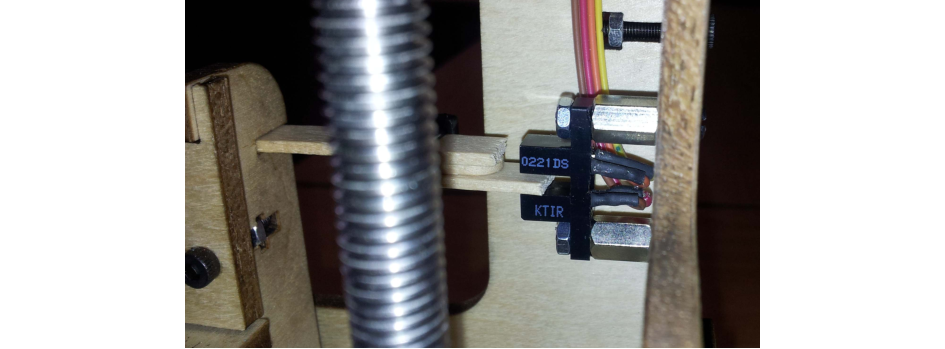
\includegraphics[width=1\textwidth]{diagrams/endstopInstalled.pdf}
				\caption{Photo-interrupter endstop being interrupted by the X-axis}
				\label{fig:endstopInstalled}
			\end{figure}
			
		\subsection{Power}
			
			The printer uses an ATX power supply unit (PSU) commonly found in desktop
			computers. A 20-pin connector containing both power and various control
			signals for the power supply (see table \ref{tab:atxConnectors}) is used
			to power the main board.
			
			\begin{table}[here]
				\centering
				\begin{tabular}{l l l}
					\toprule
					Signal & Colour & Notes\\
					\midrule
					Ground & Black  & \\
					+3.3V  & Orange & $\pm5\%$  Tolerance (Unused) \\
					+5V    & Red    & $\pm5\%$  Tolerance \\
					+12V   & Yellow & $\pm5\%$  Tolerance \\
					-12V   & Blue   & $\pm10\%$ Tolerance (Unused) \\
					\addlinespace
					Power Good  & Gray   & Signal asserted when all voltages are correct
					                       and stable \\
					+5V Standby & Purple & Power available at all times (Max 2A) \\
					+3.3V Sense & Brown  & Unused \\
					Power On    & Green  & Active-Low signal pulled up to +5V \\
					
					\bottomrule
				\end{tabular}
				
				\caption{20-pin ATX Connector Signals\cite{ATX}}
				\label{tab:atxConnectors}
			\end{table}
			
			The Mbed is connected to the 5V standby supply allowing it to remain
			connected to the network and power on the system on demand. The maximum
			power consumption of the Mbed is 200mA, well within the ratings of the ATX
			specification \cite{mbed}. The Mbed's on-board regulator provides a
			regulated 3.3V supply used by the Mbed and the low-power electronics
			attached to it. The 3.3V supply from the PSU is not used because the
			regulator in the Mbed offers a cleaner supply which is always available.
			
			To allow the PSU to be turned on by the Mbed, the power on signal is
			attached to a GPIO pin.  Because the Mbed is a 3.3V logic device a MOSFET
			is used to connect the 5V Power On signal to ground (thus turning on the
			Power Supply) using the 3.3V signal from the Mbed.
		
		\subsection{Ethernet}
			
			Ethernet requires relatively complex circuitry to drive it. With the
			exception of the Ethernet magnetics, this is provided on-board the Mbed. A
			jack containing the magnetics (figure \ref{fig:jackMagnetics}) was used to
			complete the system.
			
			\begin{figure}
				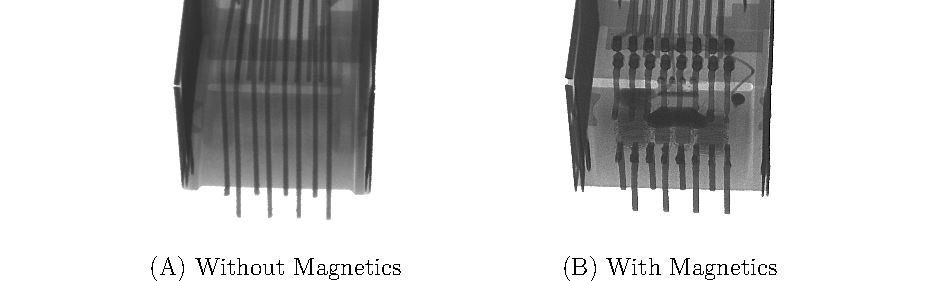
\includegraphics[width=1\textwidth]{diagrams/jackMagnetics.pdf}
				\caption{X-ray of RJ45 sockets with and without integrated magnetics
				         \cite{raspimag}}
				\label{fig:jackMagnetics}
			\end{figure}
	
	\section{Firmware}
		
		In this section the firmware for the Mbed is described, starting with the
		infrastructure required for development on FreeRTOS on the Mbed and then
		moving on to the major components of the system. Finally the safety
		precautions taken and the tools and development practices used are outlined.
		
		\subsection{FreeRTOS on the Mbed}
			
			\label{sec:compiler}
			
			The Mbed is designed for use with a web-based IDE and compiler
			\cite{mbedcompiler}. This system is not appropriate for use in the project
			as the process of uploading code to be compiled is laborious and the
			compilation options restricted.
			
			The CodeSourcery G++ None-EABI toolchain includes a GCC ARM cross-compiler,
			linker and LibC compiled for various ARM based microcontrollers. It was
			selected over closed-source alternatives because it has a large community of
			users and produces reasonable code.
			
			An unofficial port of FreeRTOS for the Mbed is available designed for the
			CodeSourcery toolchain. It provides a base FreeRTOS configuration with a
			demonstration \uIP{} based web server as well as other simple operating
			system demos. Also included are headers for the ARM Cortex Microcontroller
			Software Interface Standard (CMSIS) which defines a common interface for
			ARM Cortex microcontrollers \cite{cmsis}. Finally, headers defining macros
			and pointers for all control registers in the Mbed are included.
			
			Appendix \ref{sec:compilation} contains specific compilation instructions
			for the final system with the CodeSourcery toolchain.
		
		\subsection{Temperature Control}
			
			To drive the two heaters an active-feedback loop is used where input from
			a thermistor is used to drive a heater via a MOSFET. The following
			subsections describe how analog values are read by the Mbed and the theory
			and operation of the feedback loop that controls the heaters.
			
			\subsubsection{Analog Input}
				
				The Mbed includes a 12-bit successive-approximation analog-to-digital
				converter (ADC) for reading analog values \cite{lpc1768}. The ADC uses a
				digital-to-analog converter and a comparator to binary search for an
				approximation to the analog value while the input is held constant
				(figure \ref{fig:adc}). Once an appropriate
				number of iterations of the binary search have been carried out, the
				value in the register is returned \cite{maximadc}.
				
				\begin{figure}
					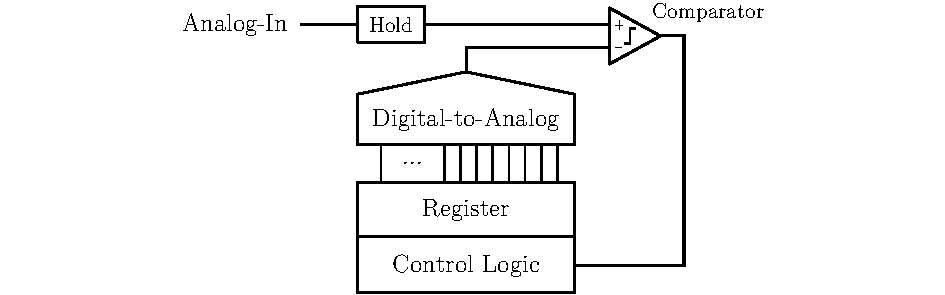
\includegraphics[width=1\textwidth]{diagrams/adc.pdf}
					\caption{Successive-approximation analog-to-digital converter}
					\label{fig:adc}
				\end{figure}
				
				The ADC sampling process takes at least $5\mu{}s$ or approximately 500
				CPU cycles therefore the CPU can carry out another task while the ADC
				process takes place \cite{lpc1768}. Though an interrupt is provided when
				the ADC completes (as well as a direct memory access (DMA) facility),
				this was not used. Instead, a slow-poll is used where the task reading
				from the ADC is suspended for a time typically adequate for ADC
				operation. The temperature sensors are sampled at an extremely low rate
				(around 2Hz) and latency is not important as changes occur very slowly.
				This system is very simple to implement with negligible overhead.
			
			\subsubsection{Heater Control Loop}
				
				A na\"{i}ve controller could simply turn on the heaters whenever the
				temperature drops below some target temperature or `set point' and then
				off when it was met or exceeded. This type of controller can cause the
				temperature to overshoot and fall below the set point as the heating and
				cooling of the system is not immediate. Instead a
				proportional-integral-derivative (PID) controller is used which can
				control heaters which takes into account such behaviours. PID
				controllers are widely used where a process which is not completely
				understood must be controlled \cite{controleng}.
				
				\begin{figure}
					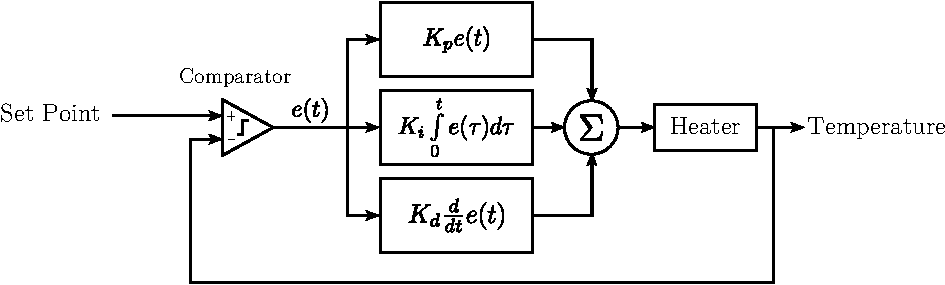
\includegraphics[width=1\textwidth]{diagrams/pid.pdf}
					\caption{PID heater controller schematic}
					\label{fig:pid}
				\end{figure}
				
				Figure \ref{fig:pid} shows a schematic of the PID controller used in the
				system. At time $t$ the comparator calculates the error, $e(t)$, between
				the actual temperature and the set point. A value is calculated from
				this error using a factor proportional to the error, the error
				accumulated over time (integral) and the error's rate of change
				(derivative). These factors are weighted by the constants $K_p$, $K_i$
				and $K_d$ respectively and the result used to control the heater. The
				three weights must be chosen manually to produce sensible behaviour.
				\S\ref{sec:pidtraning} discusses how these values were selected.
				
				The value calculated could be used to control an analog output or
				PWM\footnote{Pulse width modulation (PWM) is a method of approximating
				analog outputs by rapidly switching a signal on and off with a varying
				duty-cycle. This is cheap to implement in hardware and avoids
				inefficiencies in MOSFETs when only partially driven.} or a threshold
				value used to decide whether a heater is on or off (`bang-bang'
				control). Bang-bang control was used as the previous electronics proved
				this method to be adequate.
				
				The PID control loop is executed in its own task twice a second when
				each temperature is read and the heaters switched on and off as
				appropriate. Executing the loop more frequently would not be useful
				because of the slow rate of change in the system. Doing so would also be
				costly due to floating point calculations being carried out in software.
		
		\subsection{Stepper Control}
			
			To drive the stepper controllers, accurately timed pulses must be produced
			to cause the stepper motors to move at the correct speed. These pulses
			also need to be coherent between motors so that the three axes can move
			simultaneously to plot straight paths.
			
			\subsubsection{Principle of Operation}
			
			Before each movement begins, a periodic timer is set based on the
			frequency at which steps must occur and is used to toggle the step signal.
			This is used instead of Bresenham's line algorithm to simplify
			implementation \cite{bresenham}.  Since expensive floating point
			calculations are required for value conversion into machine units, the
			additional calculation introduced is not significant. During each timer
			tick only cheap integer operations are required.
			
			\subsubsection{Timing Constraints}
				
				The stepper controller boards are based on an Allegro A3982 stepper
				controller which defines additional timing requirements. Table
				\ref{tab:stepperTiming} gives the timing constraints for these signals.
				Figure \ref{fig:stepperWave} shows an example waveform with three
				forward steps followed by four backward steps. On the positive edge of
				the step signal the direction is sampled and the motor is stepped.
				
				\begin{figure}
					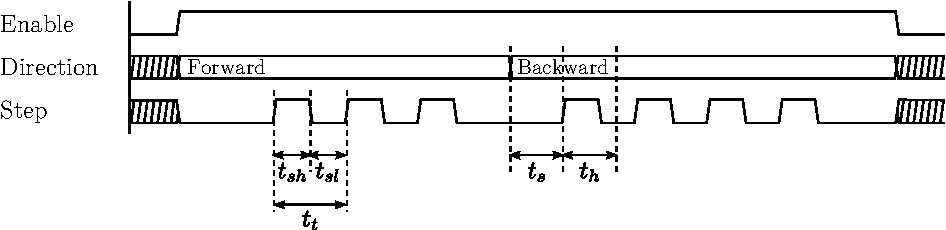
\includegraphics[width=1\textwidth]{diagrams/stepperWave.pdf}
					\caption{Stepper control signal wave diagram}
					\label{fig:stepperWave}
				\end{figure}
				
				\begin{table}
					\centering
					\begin{tabular}{l l l}
						\toprule
						Period & Meaning & Timing Constraint\\
						\midrule
						$t_{sh}$ & Step high  & $\ge 1\mu{}s$ \cite{allegro} \\
						$t_{sl}$ & Step low   & $\ge 1\mu{}s$ \cite{allegro} \\
						\addlinespace
						$t_{s}$  & Setup time & $\ge 200ns$   \cite{allegro} \\
						$t_{h}$  & Hold time  & $\ge 200ns$   \cite{allegro} \\
						\addlinespace
						$t_{t}$  & Step time  & $\ge 757\mu{}s$ (Experimentally determined) \\
						\bottomrule
					\end{tabular}
					
					\caption{Stepper timing constraints}
					\label{tab:stepperTiming}
				\end{table}
				
				The motors in the printer add an additional timing constraint, $t_t$,
				due the limit on how often they can step defined by the mechanical
				properties of the printer. This is important because the faster the
				stepper is driven, the less torque is available and so the stepper may
				miss steps and fail to move.
			
			\subsubsection{Timer Requirements}
				
				If a stepper is set to run at its maximum speed, steps will be $757\us$
				apart meaning that the signal must be toggled every $379\us$.  Therefore
				the output signals may change at up to $1.32\kHz$.
				
				FreeRTOS provides timing guarantees for scheduling arbitrary delays
				within tasks. Unfortunately, this uses the system timer which ticks at
				$1\kHz$ which is too far low for the frequencies such as those discussed
				above. 
				
				According to the Nyquist-Shannon sampling theorem a frequency of $f\Hz$
				can only be generated by a timer running at $> 2f\Hz$. This means the
				timer resolution must be above $2 \times 1.32\kHz = 2.64\kHz$
				\cite{shannon}. Figure \ref{fig:nyquist} shows `aliasing' caused by
				trying to reproduce a signal at $\frac{2}{3}$ ($> \frac{1}{2}$) the
				frequency of the timer where whole cycles are missing in the output.
				
				\begin{figure}
					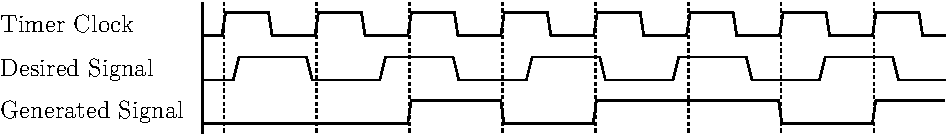
\includegraphics[width=1\textwidth]{diagrams/nyquist.pdf}
					\caption{Nyquist-Shannon sampling theorem example with high-frequency
					signal}
					\label{fig:nyquist}
				\end{figure}
				
				The effect of sampling artefacts can cause further inaccuracies. Figure
				\ref{fig:artefacts} shows a signal below $\frac{1}{2}$ of the sampling
				frequency displaying such artefacts. In the worst case when sampling at
				$f\Hz$, a signal change may be $\frac{1}{f}\s$ late. Therefore,
				increasing the sampling frequency decreases the error introduced by such
				artefacts.
				
				\begin{figure}
					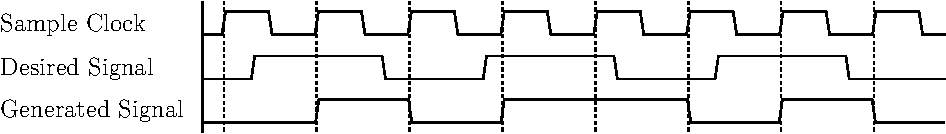
\includegraphics[width=1\textwidth]{diagrams/artefacts.pdf}
					\caption{Example of sampling artefacts}
					\label{fig:artefacts}
				\end{figure}
				
				High print quality depends on smooth, even steps, as a result, the timer
				resolution must be not only above $2.64\kHz$ due to the Nyquist-Shannon
				sampling theorem but also be high enough to reduce sampling artefacts to
				an acceptable level. If errors due to artefacts are to be reduced in the
				worst case to, for example, one-hundredth of the step period then a
				frequency of $264\kHz$ is needed.
				
				Increasing the speed of the system timer to such a frequency would make
				the overhead of the scheduler unacceptable and so the FreeRTOS timer
				cannot be used. Instead a hardware timer which interrupts the
				microcontroller causing a light weight interrupt service routine (ISR)
				to run will be needed.
				
				Because the Mbed only provides a limited number of hardware timers, just
				one is used to control all three steppers. As each stepper may not be in
				phase, the time between signals being produced for each stepper can
				become very small, even when the step period is large. This is another
				example of a sampling artefact where the resulting errors are at worst
				$\frac{1}{f}\s$ for a timer running at $f\Hz$. Because the timer is
				already sufficiently fast to make such errors insignificant, no extra
				precision is required when sharing a timer.
				
				The timers provided on board the Mbed consist of a register comparator
				and counter which is incremented by the system clock after being passed
				through a clock divider (figure \ref{fig:timerArch}). The timer was
				configured such that when the counter matches the value in the register,
				the counter is reset and the CPU is interrupted. The timer was
				configured to run at $1\MHz$ which exceeds the $264\kHz$ requirement
				calculated above with some additional margin.
				
				\begin{figure}
					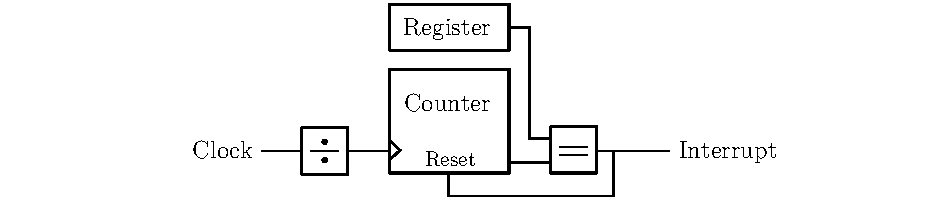
\includegraphics[width=1\textwidth]{diagrams/timerArch.pdf}
					\caption{Mbed timer architecture}
					\label{fig:timerArch}
				\end{figure}
				
				The ISR for the timer interrupt determines for each stepper, whether its
				step signal should be toggled and calculates how long until another
				interrupt is required. The timer compare register is updated, the ISR
				returns and normal program execution resumes.
				
				GCC generates approximately 100 instructions for the ISR taking an
				estimated 250 cycles to execute\footnote{Estimate based on informal
				analysis of the generated assembly code}. Assuming the CPU executes one
				instruction per cycle at $100\MHz$ the amount of CPU time used by the
				ISR in the worst case can be calculated as follows:
				\begin{equation}
					\textrm{Overhead} =
					\frac{\textrm{Interrupts Per Seccond} \times \textrm{ISR Cycles}}
					     {\textrm{Cycles Per Seccond}} =
					\frac{(1.32\times10^3) \times 250}
					     {100\times10^6} = 0.33\%
				\end{equation}
				
				This design results in very little overhead in the system but provides
				very accurately signals to the stepper motors.
			
			\subsubsection{Usage}
				
				An API is provided which allows a number of steps in a given direction
				with a specified period to be sent to a stepper motor. To allow
				sequences of coherent movements to be made, a method which blocks until
				all steps have been completed is also provided. This method uses a
				semaphore which is released by the ISR when all steps have been
				completed. This is also used to temporarily give a higher priority to
				the controlling task during which time the next sequence of steps
				can be started immediately.
		
		\subsection{G-Code Interpreter}
			
			In this subsection there is a discussion of the selection of G-code
			features implemented by the system. Following this, the implementation of
			the parser and interpreter is described.
			
			\subsubsection{Feature Subset Selection}
				
				G-code interpreters support a large variety of features ranging from
				comments and instructions which return data to error checking. As well
				as various language features, the actions available and their precise
				behaviours differ.
				
				To keep the system as simple (and fast) as possible, only features and
				actions required to support the output of Skeinforge's G-code generator
				were implemented.  The resulting language simply supports comments and
				writing to registers.  The syntax supported is given in Backus-Naur Form
				(BNF) in appendix \ref{sec:gcodebnf}.
				
				Actions (and their treatment of registers) were also selected based on the
				output of Skeinforge and include:
				\begin{itemize}
					\item Unit selection
					\item Calibration
					\item Movement
					\item Motor control
					\item Power control
					\item Temperature control
					\item Delays
				\end{itemize}
				A complete description of the actions supported is given in appendix
				\ref{sec:gcodeactions}.
			
			\subsubsection{Parsing}
				
				The G-code subset supported is very simple and so a small parser was
				implemented by hand rather than using a standard parser generator such
				as GNU Bison. Such tools also generate code that is not optimised for
				running on a microcontroller in a real-time environment and would have
				been time consuming to learn.
				
				A simple state machine was built which parses and executes the G-code
				setting and reading registers as described in \S\ref{ref:gcodemachine}.
				When unexpected characters or register values are encountered a flag is
				set and the parser continues from the next character or instruction.
				
				Once each instruction is parsed and the register values set, the values
				are converted into machine units. For example, movements are converted
				into relative movements measured in stepper motor steps and speeds
				converted into step periods measured in timer ticks. These low-level
				commands are then added to the command buffer to be executed by the
				printer controller.
		
		\subsection{Printer Controller}
			
			The printer controller uses a FreeRTOS queue in a high priority task to
			buffer low-level commands from the G-code interpreter. The controller
			consists of a simple loop which executes each command requiring minimal
			processing. As a result, this task spends most of its time blocked waiting
			for actions to complete but responds quickly when required.
		
		\subsection{Network Interface}
			
			The network interface consists of two services built on the \uIP{} stack:
			a G-code transmission interface and a status monitoring interface. \uIP{}
			provides a simple API for sending and receiving data over TCP and UDP
			within applications built within its protosocket and protothread
			frameworks \cite{uIP}.
			
			Protothreads are extremely lightweight threads using cooperative
			multitasking implemented in pure C. These threads do not preserve
			registers or variables during blocking phases of execution and use minimal
			system resources. Protosockets are a simplified UNIX-style socket
			interface built on protothreads. These libraries are designed with
			extremely low-power microcontrollers in mind.  As a result, only a minimal
			application is implemented within the \uIP{} framework which passes data
			from the network immediately to the other parts of the system.
			
			The G-code was initially implemented using TCP but a bug in \uIP{}'s flow
			control implementation meant an alternative implementation was required
			and built on UDP. The two protocols are outlined below along with an
			additional TCP interface used for reporting the system's status.
			
				\subsubsection{TCP G-code Interface}
					
					The TCP G-code interface consists of an open port listening for
					connections. Once connected a client simply sends the G-code to the
					printer and disconnects when finished. Telnet or net-cat (\verb|nc|)
					can be used to send G-code files to the printer, for example
					\begin{verbatim}
						nc 192.168.3.100 1818 -q 0 < model.gcode
					\end{verbatim}
					Where \verb|model.gcode| is the file to send and \verb|193.168.3.100|
					is the IP of the printer.
					
					As the G-code subset supported does not support return values, nothing
					is returned by the printer.
				
				\subsubsection{UDP G-code Interface}
					
					\label{sec:udpimpl}
					
					Unfortunately, as discussed in \S\ref{sec:tcpProblem}, the TCP
					implementation in \uIP{} is incorrect. Due to time constraints this
					was not fixed during the project. Instead a UDP based protocol was
					implemented.
					
					UDP provides a facility for sending datagrams containing a small
					amount of data to a remote host. These datagrams are not guaranteed to
					arrive or to arrive in the order they are sent. They do include a
					checksum and so if a datagram arrives it can be safely be assumed to
					be intact. Finally no flow-control mechanism is provided (excess
					packets are silently dropped). They are, however, lightweight and a
					good base for building custom protocols.
					
					UDP alone cannot be used to send data to the printer and simple
					protocol has been built on top which provides a communications
					channel which is
					\begin{itemize}
						\item Reliable
						\item Unidirectional
						\item Order-guaranteed
						\item Flow-controlled
					\end{itemize}
					
					Figure \ref{fig:datagram} shows the format of datagrams sent between
					the printer and sender. Datagrams are sent to the printer which
					contain a sequence number and a payload whose length can be calculated
					based on the datagram's size (contained in the UDP header). The sender
					then waits for a response from the printer containing the same
					sequence number and a window size. The printer will only respond if a
					datagram with an appropriate sequence number is received discarding
					out-of-order datagrams. If a response with a matching sequence number
					is not received by the sender within a short timeout, the datagram is
					retransmitted. This mechanism facilitates reliable, in-order
					transmission.
					
					The window size returned by the printer is used for flow control and
					is the amount of space in the G-code buffer or the maximum datagram
					size (whichever is smallest). The sender may send up to this amount of
					data to the printer in its next datagram ensuring the printer is
					always sent as much data is it can deal with. If the G-code buffer
					becomes full then the window size will become zero the sender must
					poll the printer until the window size becomes non-zero.
					
					\begin{figure}
						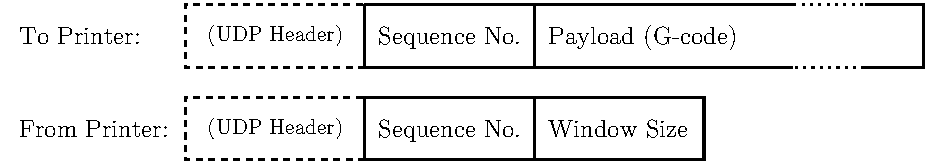
\includegraphics[width=1\textwidth]{diagrams/datagram.pdf}
						\caption{UDP G-code Sender Datagram Format}
						\label{fig:datagram}
					\end{figure}
					
					\S\ref{sec:udpPerformance} discusses the performance and practical
					implications of this protocol and the full specification is given in
					Appendix \ref{sec:udpSpec}.
			
			\subsubsection{Status Interface}
				
				\label{sec:statusInterface}
				
				A simple Telnet-compatible TCP interface (listening on port 2777) was
				implemented that can be used to request the contents of various status
				and debugging variables. As flow control was not necessary, the TCP
				implementation in \uIP{} is adequate for this purpose.
				
				The interface listens for keywords separated by white space and responds
				with tab separated data compatible with GNU Plot. For example:
				\begin{verbatim}
					tmp
					22523	22500	0	11800	12000	1
				\end{verbatim}
				The command \verb|tmp| requests current temperature information. The
				response contains the current temperature, set point (target) and
				whether the heater is on or off for the extruder and the platform.
				Temperature readings are given in degrees Celsius multiplied by 100. This is
				due to the version of LibC provided with the CodeSourcery tool chain not
				supporting printing of floating point values.
				
				A utilities for using the status monitoring facility are described in
				the next section and full documentation for the protocol is given in
				Appendix \ref{sec:statusSpec}.
	
	
	\section{Utilities}
		
		Two utilities for interacting with the printer were written in Python. The
		first, a client implementing the UDP G-code transmission protocol and, the
		second, a utility for conveniently monitoring the printer status. These
		utilities are part of the \verb|makebed.py| command.
		
		For example, the following command will stream the G-code contained in
		\verb|cube.gcode| to the printer:
		\begin{verbatim}
			makebed.py send cube.gcode
		\end{verbatim}
		
		While print jobs are running the status information can be requested or
		polled. For example:
		\begin{verbatim}
			makebed.py get temperature
		\end{verbatim}
		
		Additionally, a simple wrapper, \verb|makebed_live.sh|, is provided written
		in Bash using GNU Plot to plot various pieces of printer status information
		in real-time (figure \ref{fig:makebedlive}).
		
		\begin{figure}
			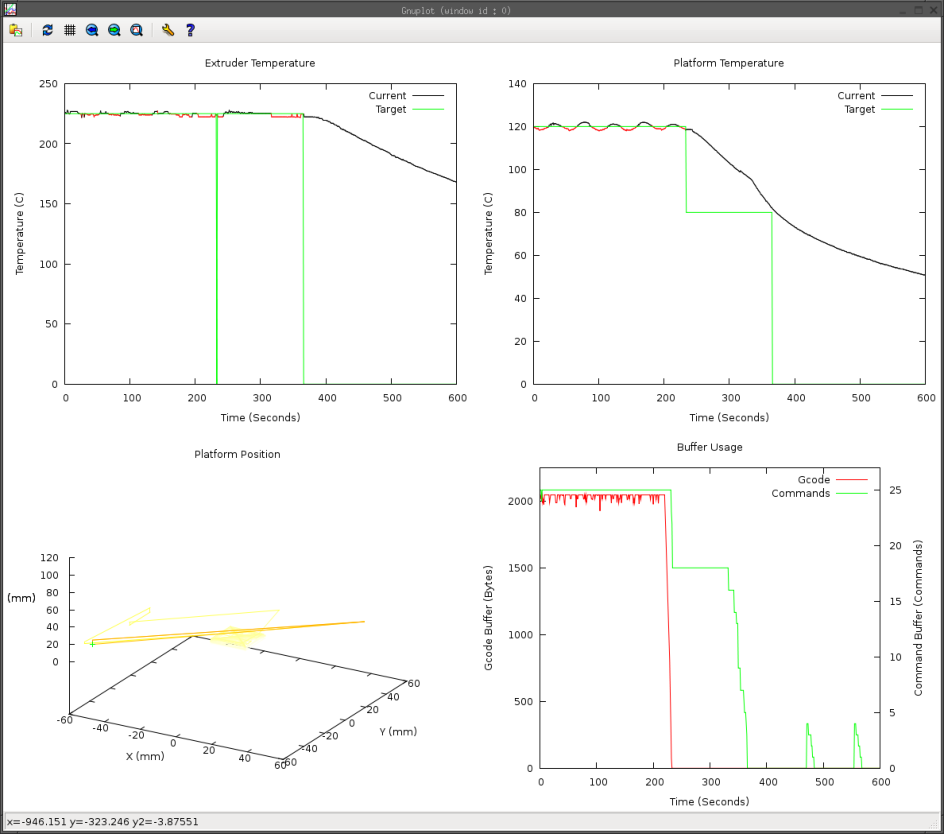
\includegraphics[width=1\textwidth]{diagrams/makebedlive.pdf}
			\caption{\texttt{makebed live.sh} screen shot}
			\label{fig:makebedlive}
		\end{figure}
		
		Usage information for the utilities can be found in Appendix
		\ref{sec:utilDoc}.
	
	\section{Safety}
		
		Because the system contains heaters and moving parts, safety was a major
		consideration when implementing the system. This section outlines the key
		features used to ensure operation is as safe as possible including
		human-interaction features and fail-safe design.
		
		\subsection{Heater Indicator LEDs}
			
			The two heaters each use an indicator LED on the microcontroller to
			indicate when the heaters are powered on. This enables an operator to
			easily and safely check the state of the heaters during operation.
		
		\subsection{Power-on Behaviour}
			
			On power-on, the PSU is not turned on and so the heaters and motors do not
			receive power. The only way to start the heaters is to open a new
			connection to the printer and send the required PSU and heater
			instructions. This design means that if the printer is powered on
			unintentionally it will not do anything unsafe. It also means that
			resetting the printer has the effect of putting it into a safe state where
			an explicit action is required to restart it.
		
		\subsection{Stop Button}
			
			The electronics connect the Mbed's reset pin to a larger and easier to
			press red button (figure \ref{fig:stop}). Because of the safe power-on
			behaviour and indifference to software failures this button can always but
			the system into a safe state.
			
			\begin{figure}
				
\includegraphics[width=1\textwidth]{diagrams/stop.pdf}
				\caption{Emergency stop/reset button}
				\label{fig:stop}
			\end{figure}
		
		\subsection{Watchdog Timer}
			
			The most safety critical software process is that of the heater
			controller. If this routine fails for any reason the heaters may become
			stuck powered on. As over-heating is not as obvious to the operator as for
			example, a jammed axis, this is a particularly dangerous fault.
			
			To catch such faults the Mbed includes a hardware watchdog timer (WDT).
			The WDT contains timer which, upon timing out, resets the system. The WDT
			must be `fed' (reset) periodically to prevent it resetting the system. To
			feed the WDT specific values must be loaded in the correct order into a
			control register. This mechanism can catch bugs which cause the routine to
			jump to a random location, block for an excessive period or otherwise
			become corrupted.
			
			The heater controller loop executes at 2Hz and the WDT is fed at the end
			of each iteration of the control loop. The WDT is set with a timeout of
			two seconds meaning that it should never come close to a timeout except in
			the event of a control loop has failure or the system resources have
			somehow become saturated.
			
			After the WDT has reset the system it enters a safe state where the
			heaters do not have power and are allowed to cool safely.
	
	\section{Methodology \& Tools}
		
		In this section the methodologies used for the implementation of the system
		are discussed followed by the choice of languages and development tools and
		why they were selected. Finally the methods used to debug the firmware
		running on the Mbed are described.
		
		\subsection{Methodology}
		
			Development followed an iterative, bottom-up process where components were
			built, tested and then integrated into the system as a whole.
			
			Prototyping was used heavily in the development of the electronics. The
			major parts of the circuit were initially prototyped on a solderless
			breadboard and powered by a bench power supply (figure
			\ref{fig:breadboard}). In these prototypes, different components could
			easily be swapped in and out of the design and measurements easily taken
			with the system running at different voltages.
			
			\begin{figure}
				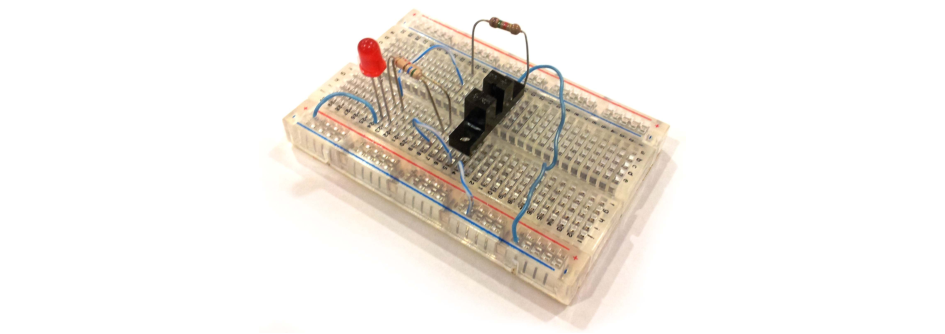
\includegraphics[width=1\textwidth]{diagrams/breadboard.pdf}
				\caption{Breadboard with a prototype end-stop circuit}
				\label{fig:breadboard}
			\end{figure}
			
			The UDP protocol was also initially prototyped using a high level language
			(Python) allowing quick development and testing. Some parts of the
			prototype were subsequently modified and used as part of the off-printer
			client software.
		
		
		\subsection{Languages}
			
			The firmware was written entirely in C. As well as a mature compiler and
			manufacturer-provided header files, C strikes a good balance between the
			availability of sensible abstractions and providing low-level access to
			the underlying hardware. Thanks to a policy of manual, static memory
			management no garbage collection or dynamic memory allocation was required
			which helps make system performance more deterministic.
			
			The off-printer utilities are written primarily in python and include a
			wrapper shell script written in Bash. These languages provide very high
			levels of abstraction simplifying and accelerating development. The
			performance costs incurred by using such languages are not relevant on a
			modern PC for the simple tasks required and so represent a good fit for
			the project.
			
		\subsection{Version Control}
			
			To track changes and keep snapshots of the project's code, Git was used
			for version control \cite{git}. Git provides facilities for quickly
			comparing versions of code. It also allows experimental copies or branches
			of the code base to be created and independently modified. Useful changes
			can be made in their own isolated branches and easily be merged back into
			the main version of the system. Changes can also quickly reverted. These
			features allowed new ideas to be created and tested without fear of
			irreversibly altering the system.
		
		\subsection{Debugging}
			
			Microcontrollers are typically debugged using a JTAG (Joint Test Action
			Group) interface which allows the microcontroller to be paused, stepped
			and examined during program execution. Unfortunately the Mbed does not
			expose this interface and so all debugging must be carried out through the
			input/output facilities provided.
			
			The port of FreeRTOS used included a demonstration web server which was
			modified during the first iteration of firmware development to allow
			program variables to be exposed through this interface. Eventually the
			demonstration code was removed and the status interface described in
			\S\ref{sec:statusInterface} was put in it's place providing equivalent
			facilities. Both interfaces allowed internal variables to be polled,
			examined and graphed on a PC.
			
			As well as the firmware itself, its interactions with the network also
			required debugging. To do this Wireshark, a network analyser was used.
			This allows the individual packets sent and received by a computer to be
			monitored, filtered and examined. It also includes protocol specific
			features such as protocol checking and protocol-specific
			statistics.
